\documentclass[9pt]{beamer}

\usepackage[utf8x]{inputenc}
\usepackage[english]{babel}
\usepackage{amsmath, amsfonts, amssymb}
\usepackage{color}
\usepackage{xcolor}
\usepackage{tikz}
\usetikzlibrary{positioning,shapes,shadows,arrows,snakes}
\usepackage{listliketab}
\usepackage{shuffle}
\usepackage{xargs}
\usepackage{multirow}
\usepackage{pgfplots}
\usepackage{csquotes}
\usepackage{verbatim}

\definecolor{BlueGreen}{cmyk}{0.85,0,0.33,0}
\definecolor{RawSienna}{cmyk}{0,0.72,1,0.45}
\definecolor{gold}{rgb}{1.,0.84,0.}
\definecolor{dgreen}{rgb}{0.,0.6,0.}

\definecolor{Noir}{RGB}{0,0,0}
\definecolor{Rouge}{RGB}{205,35,38}
\definecolor{Bleu}{RGB}{2,60,195}
\definecolor{Bleu1}{RGB}{121,176,197}
\definecolor{Vert}{RGB}{23,103,1}
\definecolor{VertOlive}{RGB}{112,141,35}
\definecolor{Orange}{RGB}{255,113,15}
\definecolor{RoseBonbon}{RGB}{249,66,158}
\definecolor{Marron}{RGB}{193,88,50}

\definecolor{mygreen}{RGB}{23,103,1}

\newcommand{\red}[1]{\textcolor{red}{#1}}
\newcommand{\blue}[1]{\textcolor{blue}{#1}}
\newcommand{\green}[1]{\textcolor{mygreen}{#1}}
\newcommand{\bluealert}[2]{\textcolor<#1>{blue}{#2}}

\tikzstyle{alert} = [color=red, line width = 1.5]
\tikzstyle{bluealert} = [color=blue, line width =1.5]
\tikzstyle{big} = [line width = 1.5]
\tikzstyle{Point} = [fill, radius=0.08]
\tikzstyle{RedPoint} = [fill, radius=0.09, color = red]


\tikzstyle{Red} = [color = red]
\tikzstyle{Blue} = [color = blue]
\tikzstyle{Green} = [color = Vert]
\tikzstyle{Gray} = [color = gray]

\definecolor{violet}{rgb}{.5,.1,.9}


\usetheme{Boadilla}
\title{Deep learning basics}
\author{G. Châtel}
\date{June 4th, 2018}

\begin{document}

%%%%%%%%%%%%%%%%%%%%%%%%%%%%%%%%%%%%%%%%%%%%%%%%%%%%%%%%%%%%%%%%%%%%%%
\begin{frame}

  \maketitle

\end{frame}
%%%%%%%%%%%%%%%%%%%%%%%%%%%%%%%%%%%%%%%%%%%%%%%%%%%%%%%%%%%%%%%%%%%%%%

%%%%%%%%%%%%%%%%%%%%%%%%%%%%%%%%%%%%%%%%%%%%%%%%%%%%%%%%%%%%%%%%%%%%%%
\begin{frame}

  \frametitle{Machine learning}

  \framesubtitle{Supervised learning}

  Machine learning is a subfield of artificial intelligence.

  \bigskip

  \begin{description}
    \item[Intuitively] We want to \emph{learn from} and \emph{make predictions
    on} data.

    \medskip

    \item[Technically] We want to build a model that approximate well
      (\textit{e.g.} minimize a loss function) an unknown function.
  \end{description}
\end{frame}
%%%%%%%%%%%%%%%%%%%%%%%%%%%%%%%%%%%%%%%%%%%%%%%%%%%%%%%%%%%%%%%%%%%%%%

%%%%%%%%%%%%%%%%%%%%%%%%%%%%%%%%%%%%%%%%%%%%%%%%%%%%%%%%%%%%%%%%%%%%%%
\begin{frame}

  \frametitle{Application examples}

  \framesubtitle{Supervised learning}

  \begin{itemize}
    \item Regression

      \smallskip

      \begin{center}
        \begin{tabular}{cc}
          \textcolor{blue}{Polynomial} & $(x, y, z) \to f(x, y, z)$ \\[0.5cm]
          \textcolor{blue}{House price} & (surface, nb rooms, city) $\to$ price \\[0.5cm]
        \end{tabular}
      \end{center}

    \item Classification

      \smallskip

      \begin{center}
        \begin{tabular}{cc}
          \textcolor{blue}{Image classification} & pixel values $\to$ cat or dog \\[0.5cm]
          \textcolor{blue}{Text classification} & list of words $\to$ spam or valid email
        \end{tabular}
      \end{center}
  \end{itemize}

\end{frame}
%%%%%%%%%%%%%%%%%%%%%%%%%%%%%%%%%%%%%%%%%%%%%%%%%%%%%%%%%%%%%%%%%%%%%%

%%%%%%%%%%%%%%%%%%%%%%%%%%%%%%%%%%%%%%%%%%%%%%%%%%%%%%%%%%%%%%%%%%%%%%
\begin{frame}

  \frametitle{Deep learning}

  \textcolor{blue}{Deep learning} is a subfield of machine learning in
  which we use \textcolor{blue}{artificial neural networks} to make
  predictions.

  \bigskip

  An artificial neural networks is a computation model \emph{loosely}
  based on the human brain. It aims to mimic electric signals
  travelling through neurons in order to make computations.

\end{frame}
%%%%%%%%%%%%%%%%%%%%%%%%%%%%%%%%%%%%%%%%%%%%%%%%%%%%%%%%%%%%%%%%%%%%%%

%%%%%%%%%%%%%%%%%%%%%%%%%%%%%%%%%%%%%%%%%%%%%%%%%%%%%%%%%%%%%%%%%%%%%%
\begin{frame}
  \frametitle{Artificial neural network}

  \framesubtitle{Neuron}

  \begin{center}
    \scalebox{0.6}{
      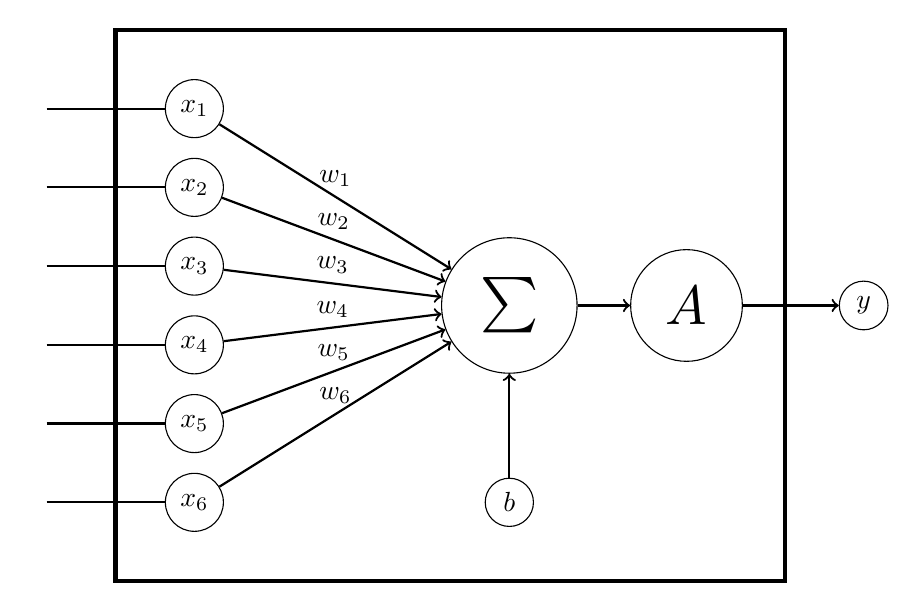
\begin{tikzpicture}
  \node (f1) at (-2, 0) {};

  \node[draw, circle] (X1) at (0, 0){
    $x_{1}$
  };

  \node (f2) at (-2, -1) {};

  \node[draw, circle] (X2) at (0, -1){
    $x_{2}$
  };

  \node (f3) at (-2, -2) {};

  \node[draw, circle] (X3) at (0, -2){
    $x_{3}$
  };

  \node (f4) at (-2, -3) {};

  \node[draw, circle] (X4) at (0, -3){
    $x_{4}$
  };

  \node (f5) at (-2, -4) {};

  \node[draw, circle] (X5) at (0, -4){
    $x_{5}$
  };

  \node (f6) at (-2, -5) {};

  \node[draw, circle] (X6) at (0, -5){
    $x_{6}$
  };

  \node[draw, circle] (bias) at (4, -5){
    $b$
  };

  \node[draw, circle] (sum) at (4, -2.5){
    \scalebox{2}{
      $\sum$
    }
  };

  \node[draw, circle] (activation) at (6.25, -2.5){
    \scalebox{2}{
      $A$
    }
  };


  %% \uncover<2->{
  %%   \node[draw, circle] (activation) at (6.25, -2.5){
  %%     \scalebox{2}{
  %%       $A$
  %%     }
  %%   };
  %% }

  \node[draw, circle] (y) at (8.5, -2.5){
    $y$
  };

  \draw[thick] (f1) -- (X1);
  \draw[thick] (f2) -- (X2);
  \draw[thick] (f3) -- (X3);
  \draw[thick] (f4) -- (X4);
  \draw[thick] (f5) -- (X5);
  \draw[thick] (f6) -- (X6);

  \draw[thick, ->] (X1) -- node [above]{$w_{1}$} (sum);
  \draw[thick, ->] (X2) -- node [above]{$w_{2}$} (sum);
  \draw[thick, ->] (X3) -- node [above]{$w_{3}$} (sum);
  \draw[thick, ->] (X4) -- node [above]{$w_{4}$} (sum);
  \draw[thick, ->] (X5) -- node [above]{$w_{5}$} (sum);
  \draw[thick, ->] (X6) -- node [above]{$w_{6}$} (sum);
  \draw[thick, ->] (bias) -- (sum);
  %% \uncover<1>{
  %%   \draw[thick, ->] (sum) -- (y);
  %% }
  %% \uncover<2->{
  %%   \draw[thick, ->] (sum) -- (activation);
  %%   \draw[thick, ->] (activation) -- (y);
  %% }
  \draw[thick, ->] (sum) -- (activation);
  \draw[thick, ->] (activation) -- (y);

  \path [ultra thick, draw] (-1, 1) -- (7.5, 1) rectangle (-1, -6) -- (7.5, -6);
\end{tikzpicture}

    }
  \end{center}

  \uncover<1->{
    \[
    A(x) = \begin{cases}
        0 & \text{if } x < 0 \\
        1 & \text{otherwise}
    \end{cases}
    \]
  }

  \uncover<2->{
    \[
    y = A(w_{1}x_{1} + w_{2}x_{2} + w_{3}x_{3} + w_{4}x_{4} + w_{5}x_{5} + w_{6}x_{6} + b)
    \]
  }
\end{frame}
%%%%%%%%%%%%%%%%%%%%%%%%%%%%%%%%%%%%%%%%%%%%%%%%%%%%%%%%%%%%%%%%%%%%%%

%%%%%%%%%%%%%%%%%%%%%%%%%%%%%%%%%%%%%%%%%%%%%%%%%%%%%%%%%%%%%%%%%%%%%%
\begin{frame}
  \frametitle{Artificial neural network}

  \framesubtitle{Network}

  \begin{center}
    \scalebox{0.7}{
      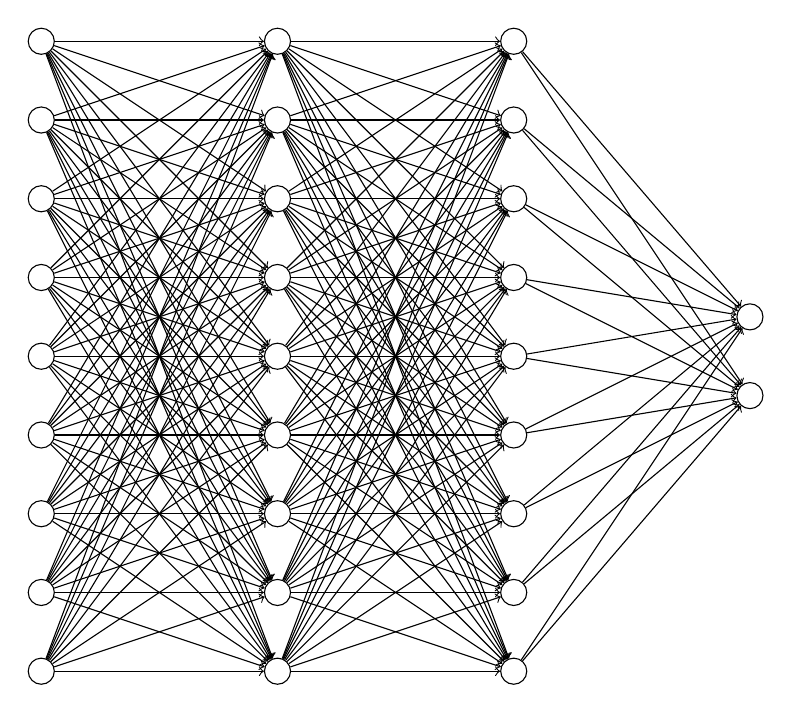
\begin{tikzpicture}[xscale = 3]
  \node[draw, circle] (N11) at (0, 0){
  };

  \node[draw, circle] (N21) at (0, -1){
  };

  \node[draw, circle] (N31) at (0, -2){
  };

  \node[draw, circle] (N41) at (0, -3){
  };

  \node[draw, circle] (N51) at (0, -4){
  };

  \node[draw, circle] (N61) at (0, -5){
  };

  \node[draw, circle] (N71) at (0, -6){
  };

  \node[draw, circle] (N81) at (0, -7){
  };

  \node[draw, circle] (N91) at (0, -8){
  };

  \node[draw, circle] (N12) at (1, 0){
  };

  \node[draw, circle] (N22) at (1, -1){
  };

  \node[draw, circle] (N32) at (1, -2){
  };

  \node[draw, circle] (N42) at (1, -3){
  };

  \node[draw, circle] (N52) at (1, -4){
  };

  \node[draw, circle] (N62) at (1, -5){
  };

  \node[draw, circle] (N72) at (1, -6){
  };

  \node[draw, circle] (N82) at (1, -7){
  };

  \node[draw, circle] (N92) at (1, -8){
  };

  \node[draw, circle] (N13) at (2, 0){
  };

  \node[draw, circle] (N23) at (2, -1){
  };

  \node[draw, circle] (N33) at (2, -2){
  };

  \node[draw, circle] (N43) at (2, -3){
  };

  \node[draw, circle] (N53) at (2, -4){
  };

  \node[draw, circle] (N63) at (2, -5){
  };

  \node[draw, circle] (N73) at (2, -6){
  };

  \node[draw, circle] (N83) at (2, -7){
  };

  \node[draw, circle] (N93) at (2, -8){
  };

  \node[draw, circle] (N14) at (3, -3.5){
  };

  \node[draw, circle] (N24) at (3, -4.5){
  };

  \draw[->] (N11) -- (N12);
  \draw[->] (N11) -- (N22);
  \draw[->] (N11) -- (N32);
  \draw[->] (N11) -- (N42);
  \draw[->] (N11) -- (N52);
  \draw[->] (N11) -- (N62);
  \draw[->] (N11) -- (N72);
  \draw[->] (N11) -- (N82);
  \draw[->] (N11) -- (N92);
  \draw[->] (N21) -- (N12);
  \draw[->] (N21) -- (N22);
  \draw[->] (N21) -- (N32);
  \draw[->] (N21) -- (N42);
  \draw[->] (N21) -- (N52);
  \draw[->] (N21) -- (N62);
  \draw[->] (N21) -- (N72);
  \draw[->] (N21) -- (N82);
  \draw[->] (N21) -- (N92);
  \draw[->] (N31) -- (N12);
  \draw[->] (N31) -- (N22);
  \draw[->] (N31) -- (N32);
  \draw[->] (N31) -- (N42);
  \draw[->] (N31) -- (N52);
  \draw[->] (N31) -- (N62);
  \draw[->] (N31) -- (N72);
  \draw[->] (N31) -- (N82);
  \draw[->] (N31) -- (N92);
  \draw[->] (N41) -- (N12);
  \draw[->] (N41) -- (N22);
  \draw[->] (N41) -- (N32);
  \draw[->] (N41) -- (N42);
  \draw[->] (N41) -- (N52);
  \draw[->] (N41) -- (N62);
  \draw[->] (N41) -- (N72);
  \draw[->] (N41) -- (N82);
  \draw[->] (N41) -- (N92);
  \draw[->] (N51) -- (N12);
  \draw[->] (N51) -- (N22);
  \draw[->] (N51) -- (N32);
  \draw[->] (N51) -- (N42);
  \draw[->] (N51) -- (N52);
  \draw[->] (N51) -- (N62);
  \draw[->] (N51) -- (N72);
  \draw[->] (N51) -- (N82);
  \draw[->] (N51) -- (N92);
  \draw[->] (N61) -- (N12);
  \draw[->] (N61) -- (N22);
  \draw[->] (N61) -- (N32);
  \draw[->] (N61) -- (N42);
  \draw[->] (N61) -- (N52);
  \draw[->] (N61) -- (N62);
  \draw[->] (N61) -- (N72);
  \draw[->] (N61) -- (N82);
  \draw[->] (N61) -- (N92);
  \draw[->] (N71) -- (N12);
  \draw[->] (N71) -- (N22);
  \draw[->] (N71) -- (N32);
  \draw[->] (N71) -- (N42);
  \draw[->] (N71) -- (N52);
  \draw[->] (N71) -- (N62);
  \draw[->] (N71) -- (N72);
  \draw[->] (N71) -- (N82);
  \draw[->] (N71) -- (N92);
  \draw[->] (N81) -- (N12);
  \draw[->] (N81) -- (N22);
  \draw[->] (N81) -- (N32);
  \draw[->] (N81) -- (N42);
  \draw[->] (N81) -- (N52);
  \draw[->] (N81) -- (N62);
  \draw[->] (N81) -- (N72);
  \draw[->] (N81) -- (N82);
  \draw[->] (N81) -- (N92);
  \draw[->] (N91) -- (N12);
  \draw[->] (N91) -- (N22);
  \draw[->] (N91) -- (N32);
  \draw[->] (N91) -- (N42);
  \draw[->] (N91) -- (N52);
  \draw[->] (N91) -- (N62);
  \draw[->] (N91) -- (N72);
  \draw[->] (N91) -- (N82);
  \draw[->] (N91) -- (N92);
  \draw[->] (N12) -- (N13);
  \draw[->] (N12) -- (N23);
  \draw[->] (N12) -- (N33);
  \draw[->] (N12) -- (N43);
  \draw[->] (N12) -- (N53);
  \draw[->] (N12) -- (N63);
  \draw[->] (N12) -- (N73);
  \draw[->] (N12) -- (N83);
  \draw[->] (N12) -- (N93);
  \draw[->] (N22) -- (N13);
  \draw[->] (N22) -- (N23);
  \draw[->] (N22) -- (N33);
  \draw[->] (N22) -- (N43);
  \draw[->] (N22) -- (N53);
  \draw[->] (N22) -- (N63);
  \draw[->] (N22) -- (N73);
  \draw[->] (N22) -- (N83);
  \draw[->] (N22) -- (N93);
  \draw[->] (N32) -- (N13);
  \draw[->] (N32) -- (N23);
  \draw[->] (N32) -- (N33);
  \draw[->] (N32) -- (N43);
  \draw[->] (N32) -- (N53);
  \draw[->] (N32) -- (N63);
  \draw[->] (N32) -- (N73);
  \draw[->] (N32) -- (N83);
  \draw[->] (N32) -- (N93);
  \draw[->] (N42) -- (N13);
  \draw[->] (N42) -- (N23);
  \draw[->] (N42) -- (N33);
  \draw[->] (N42) -- (N43);
  \draw[->] (N42) -- (N53);
  \draw[->] (N42) -- (N63);
  \draw[->] (N42) -- (N73);
  \draw[->] (N42) -- (N83);
  \draw[->] (N42) -- (N93);
  \draw[->] (N52) -- (N13);
  \draw[->] (N52) -- (N23);
  \draw[->] (N52) -- (N33);
  \draw[->] (N52) -- (N43);
  \draw[->] (N52) -- (N53);
  \draw[->] (N52) -- (N63);
  \draw[->] (N52) -- (N73);
  \draw[->] (N52) -- (N83);
  \draw[->] (N52) -- (N93);
  \draw[->] (N62) -- (N13);
  \draw[->] (N62) -- (N23);
  \draw[->] (N62) -- (N33);
  \draw[->] (N62) -- (N43);
  \draw[->] (N62) -- (N53);
  \draw[->] (N62) -- (N63);
  \draw[->] (N62) -- (N73);
  \draw[->] (N62) -- (N83);
  \draw[->] (N62) -- (N93);
  \draw[->] (N72) -- (N13);
  \draw[->] (N72) -- (N23);
  \draw[->] (N72) -- (N33);
  \draw[->] (N72) -- (N43);
  \draw[->] (N72) -- (N53);
  \draw[->] (N72) -- (N63);
  \draw[->] (N72) -- (N73);
  \draw[->] (N72) -- (N83);
  \draw[->] (N72) -- (N93);
  \draw[->] (N82) -- (N13);
  \draw[->] (N82) -- (N23);
  \draw[->] (N82) -- (N33);
  \draw[->] (N82) -- (N43);
  \draw[->] (N82) -- (N53);
  \draw[->] (N82) -- (N63);
  \draw[->] (N82) -- (N73);
  \draw[->] (N82) -- (N83);
  \draw[->] (N82) -- (N93);
  \draw[->] (N92) -- (N13);
  \draw[->] (N92) -- (N23);
  \draw[->] (N92) -- (N33);
  \draw[->] (N92) -- (N43);
  \draw[->] (N92) -- (N53);
  \draw[->] (N92) -- (N63);
  \draw[->] (N92) -- (N73);
  \draw[->] (N92) -- (N83);
  \draw[->] (N92) -- (N93);
  \draw[->] (N13) -- (N14);
  \draw[->] (N13) -- (N24);
  \draw[->] (N23) -- (N14);
  \draw[->] (N23) -- (N24);
  \draw[->] (N33) -- (N14);
  \draw[->] (N33) -- (N24);
  \draw[->] (N43) -- (N14);
  \draw[->] (N43) -- (N24);
  \draw[->] (N53) -- (N14);
  \draw[->] (N53) -- (N24);
  \draw[->] (N63) -- (N14);
  \draw[->] (N63) -- (N24);
  \draw[->] (N73) -- (N14);
  \draw[->] (N73) -- (N24);
  \draw[->] (N83) -- (N14);
  \draw[->] (N83) -- (N24);
  \draw[->] (N93) -- (N14);
  \draw[->] (N93) -- (N24);

\end{tikzpicture}

    }
  \end{center}
\end{frame}
%%%%%%%%%%%%%%%%%%%%%%%%%%%%%%%%%%%%%%%%%%%%%%%%%%%%%%%%%%%%%%%%%%%%%%

%%%%%%%%%%%%%%%%%%%%%%%%%%%%%%%%%%%%%%%%%%%%%%%%%%%%%%%%%%%%%%%%%%%%%%
%% \begin{frame}
%%   \frametitle{``Problem'' with this definition}

%%   We now have a quite complicated framework to compute
%%   \textcolor{blue}{linear functions}.

%%   \bigskip

%%   \begin{center}
%%     \begin{tabular}{cc}
%%       \textcolor{blue}{Neuron} & linear function \\
%%       \textcolor{blue}{Neural network} & linear combination of neuron outputs \\
%%     \end{tabular}
%%   \end{center}

%%   \bigskip

%%   To approximate non linear functions, we would like to have a non
%%   linear model.

%%   \bigskip

%%   \uncover<2->{\textcolor{blue}{Solution}: add nonlinearity to neurons.}
%% \end{frame}
%%%%%%%%%%%%%%%%%%%%%%%%%%%%%%%%%%%%%%%%%%%%%%%%%%%%%%%%%%%%%%%%%%%%%%

%%%%%%%%%%%%%%%%%%%%%%%%%%%%%%%%%%%%%%%%%%%%%%%%%%%%%%%%%%%%%%%%%%%%%%
%% \begin{frame}
%%   \frametitle{Neuron with activation}

%%   \begin{center}
%%     \scalebox{0.6}{
%%       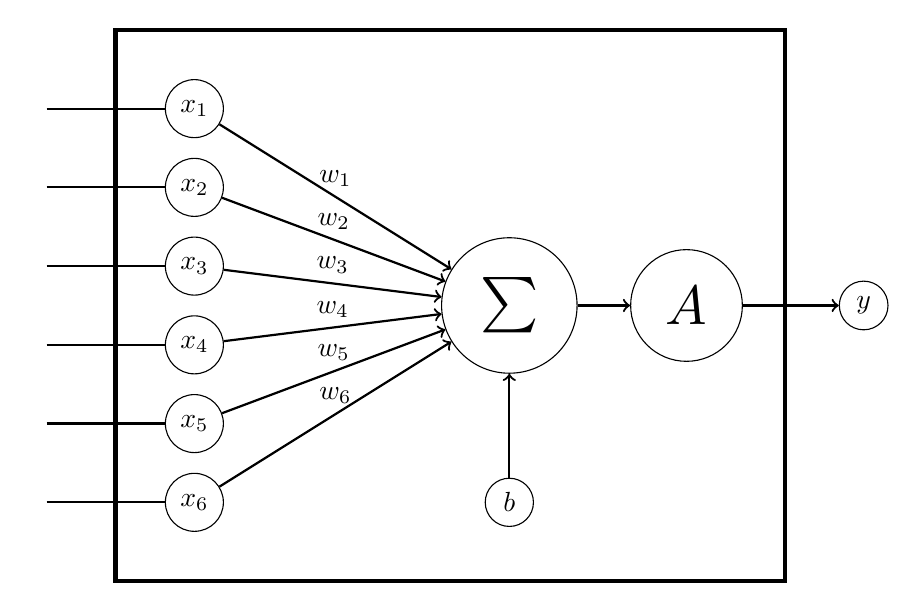
\begin{tikzpicture}
  \node (f1) at (-2, 0) {};

  \node[draw, circle] (X1) at (0, 0){
    $x_{1}$
  };

  \node (f2) at (-2, -1) {};

  \node[draw, circle] (X2) at (0, -1){
    $x_{2}$
  };

  \node (f3) at (-2, -2) {};

  \node[draw, circle] (X3) at (0, -2){
    $x_{3}$
  };

  \node (f4) at (-2, -3) {};

  \node[draw, circle] (X4) at (0, -3){
    $x_{4}$
  };

  \node (f5) at (-2, -4) {};

  \node[draw, circle] (X5) at (0, -4){
    $x_{5}$
  };

  \node (f6) at (-2, -5) {};

  \node[draw, circle] (X6) at (0, -5){
    $x_{6}$
  };

  \node[draw, circle] (bias) at (4, -5){
    $b$
  };

  \node[draw, circle] (sum) at (4, -2.5){
    \scalebox{2}{
      $\sum$
    }
  };

  \node[draw, circle] (activation) at (6.25, -2.5){
    \scalebox{2}{
      $A$
    }
  };


  %% \uncover<2->{
  %%   \node[draw, circle] (activation) at (6.25, -2.5){
  %%     \scalebox{2}{
  %%       $A$
  %%     }
  %%   };
  %% }

  \node[draw, circle] (y) at (8.5, -2.5){
    $y$
  };

  \draw[thick] (f1) -- (X1);
  \draw[thick] (f2) -- (X2);
  \draw[thick] (f3) -- (X3);
  \draw[thick] (f4) -- (X4);
  \draw[thick] (f5) -- (X5);
  \draw[thick] (f6) -- (X6);

  \draw[thick, ->] (X1) -- node [above]{$w_{1}$} (sum);
  \draw[thick, ->] (X2) -- node [above]{$w_{2}$} (sum);
  \draw[thick, ->] (X3) -- node [above]{$w_{3}$} (sum);
  \draw[thick, ->] (X4) -- node [above]{$w_{4}$} (sum);
  \draw[thick, ->] (X5) -- node [above]{$w_{5}$} (sum);
  \draw[thick, ->] (X6) -- node [above]{$w_{6}$} (sum);
  \draw[thick, ->] (bias) -- (sum);
  %% \uncover<1>{
  %%   \draw[thick, ->] (sum) -- (y);
  %% }
  %% \uncover<2->{
  %%   \draw[thick, ->] (sum) -- (activation);
  %%   \draw[thick, ->] (activation) -- (y);
  %% }
  \draw[thick, ->] (sum) -- (activation);
  \draw[thick, ->] (activation) -- (y);

  \path [ultra thick, draw] (-1, 1) -- (7.5, 1) rectangle (-1, -6) -- (7.5, -6);
\end{tikzpicture}

%%     }
%%   \end{center}

%%   \uncover<2->{
%%     \[
%%     A(x) = \begin{cases}
%%         0 & \text{if } x < 0 \\
%%         1 & \text{otherwise}
%%     \end{cases}
%%     \]
%%   }

%%   \uncover<3->{
%%     \[
%%     y = A(w_{1}x_{1} + w_{2}x_{2} + w_{3}x_{3} + w_{4}x_{4} + w_{5}x_{5} + w_{6}x_{6} + b)
%%     \]
%%   }
%% \end{frame}
%%%%%%%%%%%%%%%%%%%%%%%%%%%%%%%%%%%%%%%%%%%%%%%%%%%%%%%%%%%%%%%%%%%%%%

%%%%%%%%%%%%%%%%%%%%%%%%%%%%%%%%%%%%%%%%%%%%%%%%%%%%%%%%%%%%%%%%%%%%%%
\begin{frame}
  \frametitle{Computation example}

  \framesubtitle{Binary AND gate}

  \begin{center}
    \scalebox{1}{
      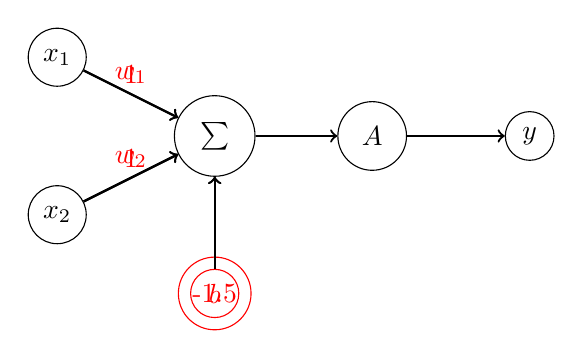
\begin{tikzpicture}[xscale = 2, yscale = 2]
  \node[draw, circle] (X1) at (0, 0){
    $x_{1}$
  };

  \node[draw, circle] (X2) at (0, -1){
    $x_{2}$
  };

  \uncover<1>{
    \node[draw, circle, red] (bias) at (1, -1.5){
      $b$
    };
  }

  \uncover<2->{
    \node[draw, circle, red] (biasVal) at (1, -1.5){
      -1.5
    };
  }

  \node[draw, circle] (sum) at (1, -0.5){
    \scalebox{1}{
      $\sum$
    }
  };

  \node[draw, circle] (activation) at (2, -0.5){
    \scalebox{1}{
      $A$
    }
  };

  \node[draw, circle] (y) at (3, -0.5){
    $y$
  };

  \uncover<1>{
    \draw[thick, ->] (X1) -- node [above, red]{$w_{1}$} (sum);
    \draw[thick, ->] (X2) -- node [above, red]{$w_{2}$} (sum);
    \draw[thick, ->] (bias) -- (sum);
  }

  \uncover<2->{
    \draw[thick, ->] (biasVal) -- (sum);
    \draw[thick, ->] (X1) -- node [above, red]{1} (sum);
    \draw[thick, ->] (X2) -- node [above, red]{1} (sum);
  }

  \draw[thick, ->] (sum) -- (activation);
  \draw[thick, ->] (activation) -- (y);
\end{tikzpicture}

    }
  \end{center}

  We want to set $w_{1}, w_{2}$ and $b$ such that:

  \[
  A(w_{1}x_{1} + w_{2}x_{2} + b) = x_{1} \text{ AND } x_{2}
  \]

  \uncover<3->{
    \[
    x_{0} = 0, x_{1} = 1. \quad y = A(0 + 1 - 1.5) = A(-0.5) = 0
    \]
  }

  \uncover<4->{
    \[
    x_{0} = 1, x_{1} = 1. \quad y = A(1 + 1 - 1.5) = A(0.5) = 1
    \]
  }
\end{frame}
%%%%%%%%%%%%%%%%%%%%%%%%%%%%%%%%%%%%%%%%%%%%%%%%%%%%%%%%%%%%%%%%%%%%%%

%%%%%%%%%%%%%%%%%%%%%%%%%%%%%%%%%%%%%%%%%%%%%%%%%%%%%%%%%%%%%%%%%%%%%%
%% \begin{frame}
%%   \frametitle{Computation example}

%%   \framesubtitle{Binary XOR gate}

%%   \begin{center}
%%     \scalebox{0.7}{
%%       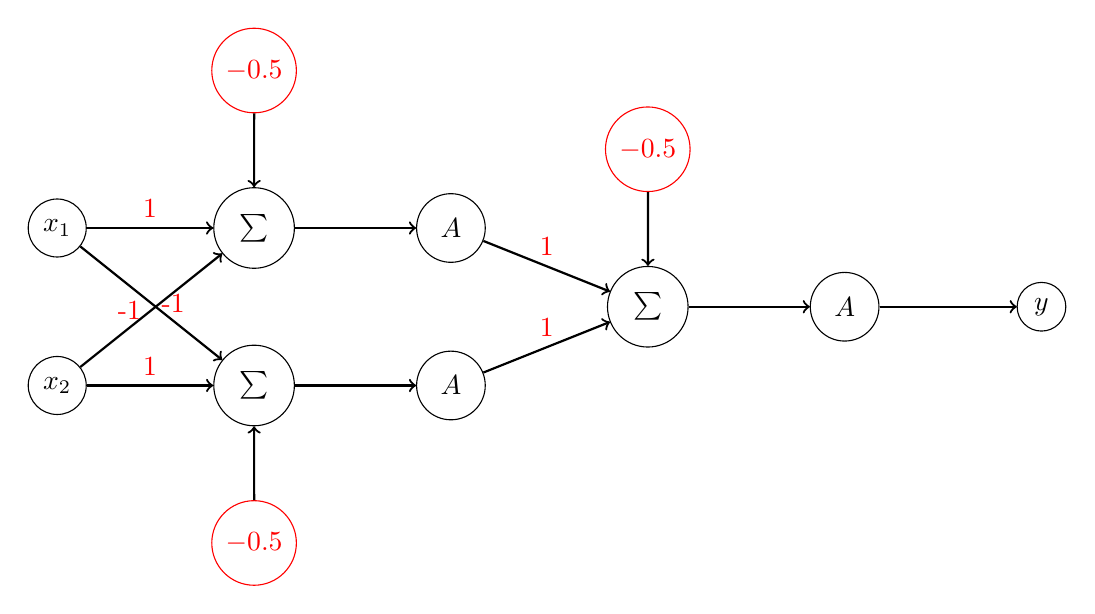
\begin{tikzpicture}[xscale = 2.5, yscale = 2]
  \node[draw, circle] (X1) at (0, 0){
    $x_{1}$
  };

  \node[draw, circle] (X2) at (0, -1){
    $x_{2}$
  };

  \node[draw, circle] (sum1) at (1, 0){
    \scalebox{1}{
      $\sum$
    }
  };

  \node[draw, circle] (act1) at (2, 0){
    \scalebox{1}{
      $A$
    }
  };

  \node[draw, circle] (sum2) at (1, -1){
    \scalebox{1}{
      $\sum$
    }
  };

  \node[draw, circle] (act2) at (2, -1){
    \scalebox{1}{
      $A$
    }
  };

  \node[draw, circle] (sum3) at (3, -0.5){
    \scalebox{1}{
      $\sum$
    }
  };

  \node[draw, circle] (act3) at (4, -0.5){
    \scalebox{1}{
      $A$
    }
  };

  \node[draw, circle, red] (bias1) at (1, 1){
    $-0.5$
  };

  \node[draw, circle, red] (bias2) at (1, -2){
    $-0.5$
  };

  \node[draw, circle, red] (bias3) at (3, 0.5){
    $-0.5$
  };

  \node[draw, circle] (y) at (5, -0.5) {
    $y$
  };

  \draw[thick, ->] (X1) -- node [above, red]{1} (sum1);
  \draw[thick, ->] (X1) -- node [below, right, red]{-1} (sum2);

  \draw[thick, ->] (X2) -- node [above, left, red]{-1} (sum1);
  \draw[thick, ->] (X2) -- node [above, red]{1} (sum2);

  \draw[thick, ->] (bias1) -- (sum1);
  \draw[thick, ->] (bias2) -- (sum2);
  \draw[thick, ->] (bias3) -- (sum3);

  \draw[thick, ->] (sum1) -- (act1);
  \draw[thick, ->] (act1) -- node[above, red]{1} (sum3);
  \draw[thick, ->] (sum2) -- (act2);
  \draw[thick, ->] (act2) -- node[above, red]{1} (sum3);
  \draw[thick, ->] (sum3) -- (act3);
  \draw[thick, ->] (act3) -- (y);
\end{tikzpicture}

%%     }
%%   \end{center}
%% \end{frame}
%%%%%%%%%%%%%%%%%%%%%%%%%%%%%%%%%%%%%%%%%%%%%%%%%%%%%%%%%%%%%%%%%%%%%%

%%%%%%%%%%%%%%%%%%%%%%%%%%%%%%%%%%%%%%%%%%%%%%%%%%%%%%%%%%%%%%%%%%%%%%
\begin{frame}
  \frametitle{Model complexity}

  One way to measure the complexity of a neural network is its number
  of parameters.

  \bigskip

  \begin{itemize}
    \uncover<2->{
    \item AND network: 3 parameters
    }
    \bigskip
    \uncover<3->{
    \item dogs vs cats pictures (VGG16 network): 138,357,544 parameters
    }
  \end{itemize}

  %% \bigskip
  %% \uncover<4->{We should probably look for a way to tune these
  %%   parameters automatically otherwise it is going to get
  %%   \emph{really} boring \emph{really} quickly.}
\end{frame}
%%%%%%%%%%%%%%%%%%%%%%%%%%%%%%%%%%%%%%%%%%%%%%%%%%%%%%%%%%%%%%%%%%%%%%

%%%%%%%%%%%%%%%%%%%%%%%%%%%%%%%%%%%%%%%%%%%%%%%%%%%%%%%%%%%%%%%%%%%%%%
%% \begin{frame}
%%   \frametitle{Parameter tuning}

%%   \framesubtitle{Line approximation}

%%   We have a few sample points and we want to find a line that
%%   approximate these points.

%%   \begin{center}
%%     \scalebox{0.8}{
%%       \begin{tikzpicture}[xscale = 3.5, yscale=3.5]
  \foreach \Point in { (0.418313, 0.604578), (0.196620, 0.549155),
    (0.734198, 0.683549), (0.767944, 0.691986), (0.212015, 0.553004),
    (0.866296, 0.716574), (0.741085, 0.685271), (0.091187, 0.522797),
    (0.957083, 0.739271), (0.400345, 0.600086), (0.110229, 0.527557),
    (0.628896, 0.657224), (0.079816, 0.519954), (0.585337, 0.646334),
    (0.240140, 0.560035), (0.712331, 0.678083), (0.810917, 0.702729),
    (0.262672, 0.565668), (0.690066, 0.672516), (0.871858, 0.717964),
    (0.444774, 0.611194), (0.021740, 0.505435), (0.308306, 0.577077),
    (0.055931, 0.513983), (0.343537, 0.585884), (0.007552, 0.501888),
    (0.614842, 0.653711), (0.343214, 0.585804), (0.627016, 0.656754),
    (0.951821, 0.737955) }{ 
    \node at \Point {
      \textbullet
    }; 
  }

  \draw[->] (0, 0) -- (1.2, 0) node[right] {$x$};
  \draw[->] (0, 0) -- (0, 1.2) node[above] {$y$};
  \draw (1, 0.25pt) -- (1, -0.5pt) node[anchor = north]{1};
  \draw (0.25pt, 1) -- (-0.5pt, 1) node[anchor = east]{1};
\end{tikzpicture}

%%     }
%%   \end{center}

%%   Our model is just a line

%%   \[
%%   y_{pred} = \textcolor{red}{a}x + \textcolor{red}{b}
%%   \]

%%   \bigskip

%%   We want to find $a$ and $b$ to best match our samples.

%% \end{frame}
%%%%%%%%%%%%%%%%%%%%%%%%%%%%%%%%%%%%%%%%%%%%%%%%%%%%%%%%%%%%%%%%%%%%%%

%%%%%%%%%%%%%%%%%%%%%%%%%%%%%%%%%%%%%%%%%%%%%%%%%%%%%%%%%%%%%%%%%%%%%%
%% \begin{frame}
%%   \frametitle{Parameter tuning}

%%   \framesubtitle{Gradient descent}

%%   First we have a define a \textcolor{blue}{loss} that measures how
%%   good our predictions are.

%%   \[
%%   l(x, y, a, b) = (y - y_{pred})^{2} = (y - (a x + b))^{2}
%%   \]

%%   \bigskip

%%   and now, we compute how the loss is affected by small changes of $a$ and
%%   $b$:

%%   \medskip

%%   \[
%%   \frac{dl}{da} = 2 x (ax + b - y) \qquad \qquad \frac{dl}{db} = 2 (ax + b - y)
%%   \]
%% \end{frame}
%%%%%%%%%%%%%%%%%%%%%%%%%%%%%%%%%%%%%%%%%%%%%%%%%%%%%%%%%%%%%%%%%%%%%%

%%%%%%%%%%%%%%%%%%%%%%%%%%%%%%%%%%%%%%%%%%%%%%%%%%%%%%%%%%%%%%%%%%%%%%
%% \begin{frame}
%%   \frametitle{Parameter tuning}

%%   \framesubtitle{Gradient descent}

%%   We start with random values: $a = -2$ and $b = 1$

%%   \begin{center}
%%     \scalebox{0.7}{
%%       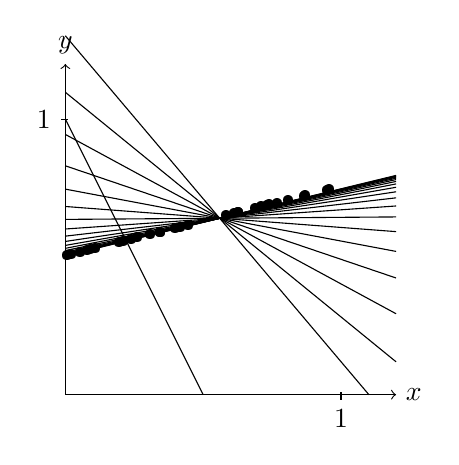
\begin{tikzpicture}[xscale = 3.5, yscale=3.5]
  \foreach \Point in { (0.418313, 0.604578), (0.196620, 0.549155),
    (0.734198, 0.683549), (0.767944, 0.691986), (0.212015, 0.553004),
    (0.866296, 0.716574), (0.741085, 0.685271), (0.091187, 0.522797),
    (0.957083, 0.739271), (0.400345, 0.600086), (0.110229, 0.527557),
    (0.628896, 0.657224), (0.079816, 0.519954), (0.585337, 0.646334),
    (0.240140, 0.560035), (0.712331, 0.678083), (0.810917, 0.702729),
    (0.262672, 0.565668), (0.690066, 0.672516), (0.871858, 0.717964),
    (0.444774, 0.611194), (0.021740, 0.505435), (0.308306, 0.577077),
    (0.055931, 0.513983), (0.343537, 0.585884), (0.007552, 0.501888),
    (0.614842, 0.653711), (0.343214, 0.585804), (0.627016, 0.656754),
    (0.951821, 0.737955) }{ 
    \node at \Point {
      \textbullet
    }; 
  }

  \draw[->] (0, 0) -- (1.2, 0) node[right] {$x$};
  \draw[->] (0, 0) -- (0, 1.2) node[above] {$y$};
  \draw (1, 0.25pt) -- (1, -0.5pt) node[anchor = north]{1};
  \draw (0.25pt, 1) -- (-0.5pt, 1) node[anchor = east]{1};
  \uncover<1>{\draw (0.000000, 1.000000) -- (0.500000, 0.000000);}
  \uncover<2>{\draw (0.000000, 1.302205) -- (1.101420, 0.000000);}
  \uncover<3>{\draw (0.000000, 1.097310) -- (1.200000, 0.119256);}
  \uncover<4>{\draw (0.000000, 0.944298) -- (1.200000, 0.293644);}
  \uncover<5>{\draw (0.000000, 0.830482) -- (1.200000, 0.423357);}
  \uncover<6>{\draw (0.000000, 0.745822) -- (1.200000, 0.519842);}
  \uncover<7>{\draw (0.000000, 0.682850) -- (1.200000, 0.591610);}
  \uncover<8>{\draw (0.000000, 0.636009) -- (1.200000, 0.644993);}
  \uncover<9>{\draw (0.000000, 0.601168) -- (1.200000, 0.684702);}
  \uncover<10>{\draw (0.000000, 0.575251) -- (1.200000, 0.714238);}
  \uncover<11>{\draw (0.000000, 0.555974) -- (1.200000, 0.736207);}
  \uncover<12>{\draw (0.000000, 0.541635) -- (1.200000, 0.752549);}
  \uncover<13>{\draw (0.000000, 0.530970) -- (1.200000, 0.764705);}
  \uncover<14>{\draw (0.000000, 0.523036) -- (1.200000, 0.773746);}
  \uncover<15>{\draw (0.000000, 0.517135) -- (1.200000, 0.780472);}
  \uncover<16>{\draw (0.000000, 0.512745) -- (1.200000, 0.785474);}
  \uncover<17>{\draw (0.000000, 0.509480) -- (1.200000, 0.789195);}
  \uncover<18>{\draw (0.000000, 0.507052) -- (1.200000, 0.791963);}
  \uncover<19>{\draw (0.000000, 0.505245) -- (1.200000, 0.794022);}
  \uncover<20>{\draw (0.000000, 0.503902) -- (1.200000, 0.795553);}
\end{tikzpicture}

%%     }
%%   \end{center}

%%   Then, we compute the average of the gradient along all $(x, y)$ couples

%%   \begin{overprint}
%%     \onslide<1> \[ a = -2.00 \quad b = 1.00 \quad \overline{\frac{dl}{da}} = -1.07 \quad \overline{\frac{dl}{db}} = -1.37 \quad \overline{l(x, y, a, b)} = 0.860367 \]
%%     \onslide<2> \[ a = -1.18 \quad b = 1.30 \quad \overline{\frac{dl}{da}} = -0.17 \quad \overline{\frac{dl}{db}} = 0.09 \quad \overline{l(x, y, a, b)} = 0.159420 \]
%%     \onslide<3> \[ a = -0.82 \quad b = 1.10 \quad \overline{\frac{dl}{da}} = -0.13 \quad \overline{\frac{dl}{db}} = 0.07 \quad \overline{l(x, y, a, b)} = 0.088204 \]
%%     \onslide<4> \[ a = -0.54 \quad b = 0.94 \quad \overline{\frac{dl}{da}} = -0.09 \quad \overline{\frac{dl}{db}} = 0.05 \quad \overline{l(x, y, a, b)} = 0.048802 \]
%%     \onslide<5> \[ a = -0.34 \quad b = 0.83 \quad \overline{\frac{dl}{da}} = -0.07 \quad \overline{\frac{dl}{db}} = 0.04 \quad \overline{l(x, y, a, b)} = 0.027001 \]
%%     \onslide<6> \[ a = -0.19 \quad b = 0.75 \quad \overline{\frac{dl}{da}} = -0.05 \quad \overline{\frac{dl}{db}} = 0.03 \quad \overline{l(x, y, a, b)} = 0.014939 \]
%%     \onslide<7> \[ a = -0.08 \quad b = 0.68 \quad \overline{\frac{dl}{da}} = -0.04 \quad \overline{\frac{dl}{db}} = 0.02 \quad \overline{l(x, y, a, b)} = 0.008266 \]
%%     \onslide<8> \[ a = 0.01 \quad b = 0.64 \quad \overline{\frac{dl}{da}} = -0.03 \quad \overline{\frac{dl}{db}} = 0.02 \quad \overline{l(x, y, a, b)} = 0.004573 \]
%%     \onslide<9> \[ a = 0.07 \quad b = 0.60 \quad \overline{\frac{dl}{da}} = -0.02 \quad \overline{\frac{dl}{db}} = 0.01 \quad \overline{l(x, y, a, b)} = 0.002530 \]
%%     \onslide<10> \[ a = 0.12 \quad b = 0.58 \quad \overline{\frac{dl}{da}} = -0.02 \quad \overline{\frac{dl}{db}} = 0.01 \quad \overline{l(x, y, a, b)} = 0.001400 \]
%%     \onslide<11> \[ a = 0.15 \quad b = 0.56 \quad \overline{\frac{dl}{da}} = -0.01 \quad \overline{\frac{dl}{db}} = 0.01 \quad \overline{l(x, y, a, b)} = 0.000775 \]
%%     \onslide<12> \[ a = 0.18 \quad b = 0.54 \quad \overline{\frac{dl}{da}} = -0.01 \quad \overline{\frac{dl}{db}} = 0.00 \quad \overline{l(x, y, a, b)} = 0.000429 \]
%%     \onslide<13> \[ a = 0.19 \quad b = 0.53 \quad \overline{\frac{dl}{da}} = -0.01 \quad \overline{\frac{dl}{db}} = 0.00 \quad \overline{l(x, y, a, b)} = 0.000237 \]
%%     \onslide<14> \[ a = 0.21 \quad b = 0.52 \quad \overline{\frac{dl}{da}} = 0.00 \quad \overline{\frac{dl}{db}} = 0.00 \quad \overline{l(x, y, a, b)} = 0.000131 \]
%%     \onslide<15> \[ a = 0.22 \quad b = 0.52 \quad \overline{\frac{dl}{da}} = 0.00 \quad \overline{\frac{dl}{db}} = 0.00 \quad \overline{l(x, y, a, b)} = 0.000073 \]
%%     \onslide<16> \[ a = 0.23 \quad b = 0.51 \quad \overline{\frac{dl}{da}} = 0.00 \quad \overline{\frac{dl}{db}} = 0.00 \quad \overline{l(x, y, a, b)} = 0.000040 \]
%%     \onslide<17> \[ a = 0.23 \quad b = 0.51 \quad \overline{\frac{dl}{da}} = 0.00 \quad \overline{\frac{dl}{db}} = 0.00 \quad \overline{l(x, y, a, b)} = 0.000022 \]
%%     \onslide<18> \[ a = 0.24 \quad b = 0.51 \quad \overline{\frac{dl}{da}} = 0.00 \quad \overline{\frac{dl}{db}} = 0.00 \quad \overline{l(x, y, a, b)} = 0.000012 \]
%%     \onslide<19> \[ a = 0.24 \quad b = 0.51 \quad \overline{\frac{dl}{da}} = 0.00 \quad \overline{\frac{dl}{db}} = 0.00 \quad \overline{l(x, y, a, b)} = 0.000007 \]
%%     \onslide<20> \[ a = 0.24 \quad b = 0.50 \quad \overline{\frac{dl}{da}} = 0.00 \quad \overline{\frac{dl}{db}} = 0.00 \quad \overline{l(x, y, a, b)} = 0.000004 \]
%%   \end{overprint}

%%   \bigskip

%%   And update $a$ and $b$ by substracting a small proportion of their
%%   gradient.

%% \end{frame}
%%%%%%%%%%%%%%%%%%%%%%%%%%%%%%%%%%%%%%%%%%%%%%%%%%%%%%%%%%%%%%%%%%%%%%

%%%%%%%%%%%%%%%%%%%%%%%%%%%%%%%%%%%%%%%%%%%%%%%%%%%%%%%%%%%%%%%%%%%%%%
%% \begin{frame}

%%   \frametitle{Parameter tuning}

%%   \framesubtitle{Problem with ANN}

%%   Using gradient descent, we know how to minimize (or at least reach a
%%   local minima) a differentiable function.

%%   \pause
%%   \bigskip

%%   \textcolor{red}{Problem}: The function computed by our neural network is not
%%   differentiable because of the activation function.

%%   \[
%%   A(x) = \begin{cases}
%%     0 & \text{if } x < 0 \\
%%     1 & \text{otherwise}
%%   \end{cases}
%%   \]

%%   \medskip

%%   \pause

%%   \textcolor{blue}{Solution}: We replace it by a differentiable
%%   function that does the same job.

%%   \begin{center}
%%     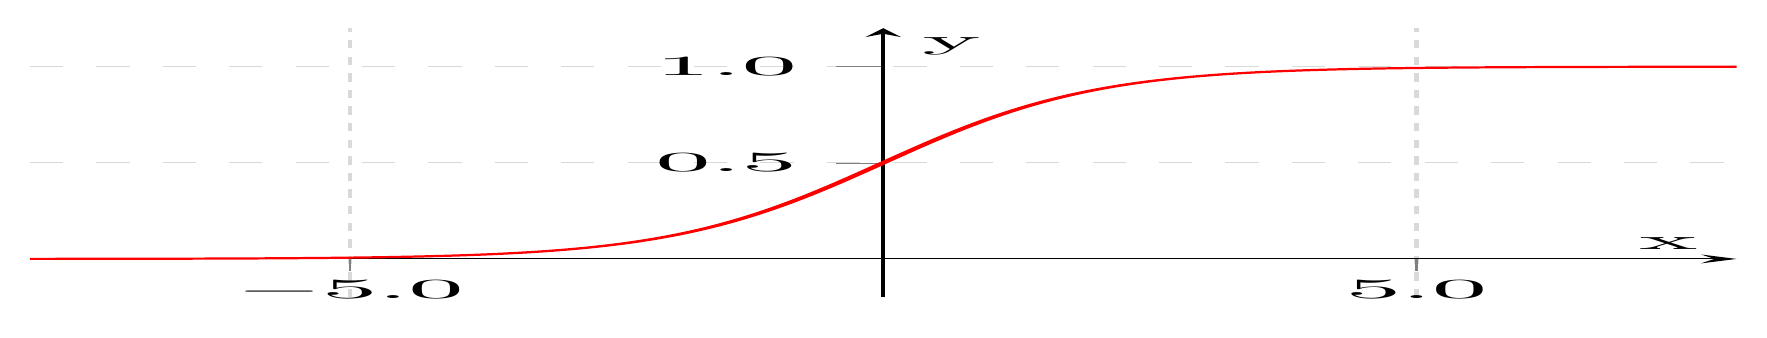
\begin{tikzpicture}[xscale = 4]
%%       \node (formula) (0, 0){
%%         \scalebox{1.3}{
%%           $A(x) = \frac{1}{1 + e^{-x}}$
%%         }
%%       } ;

%%       \node (graph) at (1, 0){
%%         \scalebox{0.6}{
%%           \begin{tikzpicture}
  \begin{axis}[
      legend pos=north west,
      axis x line=middle,
      axis y line=middle,
      x tick label style={/pgf/number format/fixed,
        /pgf/number format/fixed zerofill,
        /pgf/number format/precision=1},
      y tick label style={/pgf/number format/fixed,
        /pgf/number format/fixed zerofill,
        /pgf/number format/precision=1},
      grid = major,
      width=7cm,
      height=5cm,
      grid style={dashed, gray!30},
      xmin=-8,     % start the diagram at this x-coordinate
      xmax= 8,    % end   the diagram at this x-coordinate
      ymin= -0.2,     % start the diagram at this y-coordinate
      ymax= 1.2,   % end   the diagram at this y-coordinate
      %axis background/.style={fill=white},
      xlabel=x,
      ylabel=y,
      tick align=outside,
      enlargelimits=false]
    % plot the stirling-formulae
    \addplot[domain=-8:8, red, thick,samples=500] {1/(1+exp(-x))};
  \end{axis}
\end{tikzpicture}

%%         }
%%       };
%%     \end{tikzpicture}
%%   \end{center}
%% \end{frame}
%%%%%%%%%%%%%%%%%%%%%%%%%%%%%%%%%%%%%%%%%%%%%%%%%%%%%%%%%%%%%%%%%%%%%%

%%%%%%%%%%%%%%%%%%%%%%%%%%%%%%%%%%%%%%%%%%%%%%%%%%%%%%%%%%%%%%%%%%%%%%
%% \begin{frame}
%%   \frametitle{Convolution}

%%   \framesubtitle{Motivation}

%%   For now, our networks computes a nonlinear function of the
%%   inputs. If we work with images, it has to learn the \emph{spacial
%%     structure} of the data by itself, which takes a long time.

%%   \bigskip

%%   A nice way to help it is to build \textcolor{blue}{convolution
%%     layers} into the network.
%% \end{frame}
%%%%%%%%%%%%%%%%%%%%%%%%%%%%%%%%%%%%%%%%%%%%%%%%%%%%%%%%%%%%%%%%%%%%%%

%%%%%%%%%%%%%%%%%%%%%%%%%%%%%%%%%%%%%%%%%%%%%%%%%%%%%%%%%%%%%%%%%%%%%%
%% \begin{frame}

%%   \frametitle{Convolution}

%%   \framesubtitle{Kernel}

%%   \begin{center}
%%     \scalebox{0.55}{
%%       \includegraphics{images/kernel.jpg}
%%     }
%%   \end{center}

%%   {\small Image from \url{http://stats.stackexchange.com/}}

%% \end{frame}
%%%%%%%%%%%%%%%%%%%%%%%%%%%%%%%%%%%%%%%%%%%%%%%%%%%%%%%%%%%%%%%%%%%%%%

%%%%%%%%%%%%%%%%%%%%%%%%%%%%%%%%%%%%%%%%%%%%%%%%%%%%%%%%%%%%%%%%%%%%%%
%% \begin{frame}

%%   \frametitle{Convolution}

%%   \framesubtitle{Example: Sobel operators}

%%   \begin{center}
%%     \scalebox{0.9}{
%%       \begin{tikzpicture}[xscale = 8, yscale = 2]
  \node (dog) at (0, 0) {
    \includegraphics[width = 3cm]{images/pre_kernel.jpg}
  };
  
  \node (hori) at (1, 1) {
    \includegraphics[width = 3cm]{images/horizontal.jpg}
  };
  
  \node (vert) at (1, -1) {
    \includegraphics[width = 3cm]{images/vertical.jpg}
  };

  \draw[thick, ->] (dog) -- node [below]{$\left(\begin{matrix}-1 & 0 & 1\\ -2 & 0 & 2 \\ -1 & 0 & 1\end{matrix}\right)$} (vert);

  \draw[thick, ->] (dog) -- node [above]{$\left(\begin{matrix}-1 & -2 & -1\\ 0 & 0 & 0 \\ 1 & 2 & 1\end{matrix}\right)$} (hori);
\end{tikzpicture}

%%     }
%%   \end{center}

%%   {\small Image from \url{http://www.reddit.com/}}
%% \end{frame}
%%%%%%%%%%%%%%%%%%%%%%%%%%%%%%%%%%%%%%%%%%%%%%%%%%%%%%%%%%%%%%%%%%%%%%

%%%%%%%%%%%%%%%%%%%%%%%%%%%%%%%%%%%%%%%%%%%%%%%%%%%%%%%%%%%%%%%%%%%%%%
\begin{frame}

  \frametitle{Convolutional neural network}

  \framesubtitle{VGG network (2014)}

  \begin{center}
    \scalebox{0.5}{
      \includegraphics{images/vgg16_architecture.png}
    }
  \end{center}

  Classify natural images into 1000 categories. (92.7\% top-5
  accuracy).

  \medskip

  {\footnotesize Image from
    \url{https://www.cs.toronto.edu/~frossard/post/vgg16/}}

  \smallskip

  {\footnotesize Simonyan, K., \& Zisserman, A. (2014). Very deep
    convolutional networks for large-scale image recognition. arXiv
    preprint arXiv:1409.1556.}
\end{frame}
%%%%%%%%%%%%%%%%%%%%%%%%%%%%%%%%%%%%%%%%%%%%%%%%%%%%%%%%%%%%%%%%%%%%%%

%%%%%%%%%%%%%%%%%%%%%%%%%%%%%%%%%%%%%%%%%%%%%%%%%%%%%%%%%%%%%%%%%%%%%%
%% \begin{frame}
%%   \frametitle{Convolution}

%%   \framesubtitle{What do filter recognize?}

%%   {\small Image from \url{http://www.matthewzeiler.com/pubs/arxive2013/eccv2014.pdf}}

%%   \begin{center}
%%     \begin{overprint}
%%       \onslide<1> \includegraphics[width = 4cm]{images/cnn_vizu_l1.jpg}
%%       \onslide<2> \includegraphics[width = 11cm]{images/cnn_vizu_l2.jpg}
%%       \onslide<3> \includegraphics[width = 11cm]{images/cnn_vizu_l3.jpg}
%%       \onslide<4> \includegraphics[width = 9cm]{images/cnn_vizu_l4.jpg}
%%       \onslide<5> \includegraphics[width = 9cm]{images/cnn_vizu_l5.jpg}
%%     \end{overprint}
%%   \end{center}

%% \end{frame}
%%%%%%%%%%%%%%%%%%%%%%%%%%%%%%%%%%%%%%%%%%%%%%%%%%%%%%%%%%%%%%%%%%%%%%

%%%%%%%%%%%%%%%%%%%%%%%%%%%%%%%%%%%%%%%%%%%%%%%%%%%%%%%%%%%%%%%%%%%%%%
%% \begin{frame}

%%   \frametitle{Convolutional neural network}

%%   \framesubtitle{VGG network (2014)}

%%   \begin{center}
%%     \scalebox{0.6}{
%%       \includegraphics{images/vgg16_architecture.png}
%%     }
%%   \end{center}

%%   {\small Image from \url{https://www.cs.toronto.edu/~frossard/post/vgg16/}}
%% \end{frame}
%%%%%%%%%%%%%%%%%%%%%%%%%%%%%%%%%%%%%%%%%%%%%%%%%%%%%%%%%%%%%%%%%%%%%%

%%%%%%%%%%%%%%%%%%%%%%%%%%%%%%%%%%%%%%%%%%%%%%%%%%%%%%%%%%%%%%%%%%%%%%

%%%%%%%%%%%%%%%%%%%%%%%%%%%%%%%%%%%%%%%%%%%%%%%%%%%%%%%%%%%%%%%%%%%%%%

%%%%%%%%%%%%%%%%%%%%%%%%%%%%%%%%%%%%%%%%%%%%%%%%%%%%%%%%%%%%%%%%%%%%%%
\begin{frame}
  \frametitle{Architecture examples}

  \framesubtitle{Deep autoencoder}

  \begin{center}
    \scalebox{0.6}{
      \includegraphics{images/autoencoder.png}
    }
  \end{center}

  \medskip

  If we cut this autoencoder at the bottleneck, we get two parts: an
  encoder and a decoder. The encoder is an encoder highly specific to
  the content the network has been trained with.

  \bigskip

  {\footnotesize Hinton, G. E., \& Salakhutdinov,
    R. R. (2006). Reducing the dimensionality of data with neural
    networks. science, 313(5786), 504-507.}
\end{frame}
%%%%%%%%%%%%%%%%%%%%%%%%%%%%%%%%%%%%%%%%%%%%%%%%%%%%%%%%%%%%%%%%%%%%%%

%%%%%%%%%%%%%%%%%%%%%%%%%%%%%%%%%%%%%%%%%%%%%%%%%%%%%%%%%%%%%%%%%%%%%%
\begin{frame}
  \frametitle{Architecture examples}

  \framesubtitle{Deep autoencoder: Compression}

  \begin{center}
    \scalebox{0.3}{
      \includegraphics{images/generative_compression.png}
    }
  \end{center}

  \medskip

  If we force the output image to be realistic, we lose
  \emph{semantic information} rather than resolution.

  \bigskip

  {\footnotesize Santurkar, S., Budden, D., \& Shavit,
    N. (2017). Generative compression. arXiv preprint
    arXiv:1703.01467.}
\end{frame}
%%%%%%%%%%%%%%%%%%%%%%%%%%%%%%%%%%%%%%%%%%%%%%%%%%%%%%%%%%%%%%%%%%%%%%

%%%%%%%%%%%%%%%%%%%%%%%%%%%%%%%%%%%%%%%%%%%%%%%%%%%%%%%%%%%%%%%%%%%%%%
\begin{frame}
  \frametitle{Architecture examples}

  \framesubtitle{Drawing cleanup}

  \begin{center}
    \includegraphics[width = \linewidth]{images/drawing_simplification_example.png}
  \end{center}

  \bigskip

  {\footnotesize Simo-Serra, E., Iizuka, S., Sasaki, K., \& Ishikawa,
    H. (2016). Learning to simplify: fully convolutional networks for
    rough sketch cleanup. ACM Transactions on Graphics (TOG), 35(4),
    121.}
\end{frame}
%%%%%%%%%%%%%%%%%%%%%%%%%%%%%%%%%%%%%%%%%%%%%%%%%%%%%%%%%%%%%%%%%%%%%%

%%%%%%%%%%%%%%%%%%%%%%%%%%%%%%%%%%%%%%%%%%%%%%%%%%%%%%%%%%%%%%%%%%%%%%
%% \begin{frame}
%%   \frametitle{Architecture examples}

%%   \framesubtitle{CNN + Autoencoder network: drawing simplification}

%%   \begin{center}
%%     \includegraphics[width=\linewidth]{images/drawing_simplification.png}
%%   \end{center}

%%   Simo-Serra, Iizuka, Sasaki, Ishikawa (2016)
%% \end{frame}
%%%%%%%%%%%%%%%%%%%%%%%%%%%%%%%%%%%%%%%%%%%%%%%%%%%%%%%%%%%%%%%%%%%%%%

%%%%%%%%%%%%%%%%%%%%%%%%%%%%%%%%%%%%%%%%%%%%%%%%%%%%%%%%%%%%%%%%%%%%%%
%% \begin{frame}
%%   \frametitle{Architecture examples}

%%   \framesubtitle{Neural style}

%%   Consider an image $I$ and its image by the convolution layers of the
%%   VGG network $Conv(I)$.

%%   \pause
%%   \bigskip

%%   We can reconstruct a picture $I'$ with the same content as $I$ by
%%   applying gradient descent on the pixels in order to obtain $Conv(I)$
%%   as output, starting with white noise.

%%   \begin{center}
%%     \scalebox{0.6}{
%%       \begin{tikzpicture}
  \node (f1) at (-2, 0) {};

  \node[draw, circle] (X1) at (0, 0){
    \textcolor<3>{red}{$x_{1}$}
  };

  \node (f2) at (-2, -1) {};

  \node[draw, circle] (X2) at (0, -1){
    \textcolor<3>{red}{$x_{2}$}
  };

  \node (f3) at (-2, -2) {};

  \node[draw, circle] (X3) at (0, -2){
    \textcolor<3>{red}{$x_{3}$}
  };

  \node (f4) at (-2, -3) {};

  \node[draw, circle] (X4) at (0, -3){
    \textcolor<3>{red}{$x_{4}$}
  };

  \node (f5) at (-2, -4) {};

  \node[draw, circle] (X5) at (0, -4){
    \textcolor<3>{red}{$x_{5}$}
  };

  \node (f6) at (-2, -5) {};

  \node[draw, circle] (X6) at (0, -5){
    \textcolor<3>{red}{$x_{6}$}
  };

  \node[draw, circle] (bias) at (4, -5){
    \textcolor<2>{red}{$b$}
  };

  \node[draw, circle] (sum) at (4, -2.5){
    \scalebox{2}{
      $\sum$
    }
  };

  \uncover<2->{
    \node[draw, circle] (activation) at (6.25, -2.5){
      \scalebox{2}{
        $A$
      }
    };
  }

  \node[draw, circle] (y) at (8.5, -2.5){
    $y$
  };

  \draw[thick] (f1) -- (X1);
  \draw[thick] (f2) -- (X2);
  \draw[thick] (f3) -- (X3);
  \draw[thick] (f4) -- (X4);
  \draw[thick] (f5) -- (X5);
  \draw[thick] (f6) -- (X6);

  \draw[thick, ->] (X1) -- node [above]{\textcolor<2>{red}{$w_{1}$}} (sum);
  \draw[thick, ->] (X2) -- node [above]{\textcolor<2>{red}{$w_{2}$}} (sum);
  \draw[thick, ->] (X3) -- node [above]{\textcolor<2>{red}{$w_{3}$}} (sum);
  \draw[thick, ->] (X4) -- node [above]{\textcolor<2>{red}{$w_{4}$}} (sum);
  \draw[thick, ->] (X5) -- node [above]{\textcolor<2>{red}{$w_{5}$}} (sum);
  \draw[thick, ->] (X6) -- node [above]{\textcolor<2>{red}{$w_{6}$}} (sum);
  \draw[thick, ->] (bias) -- (sum);
  \uncover<1>{
    \draw[thick, ->] (sum) -- (y);
  }
  \uncover<2->{
    \draw[thick, ->] (sum) -- (activation);
    \draw[thick, ->] (activation) -- (y);
  }

  \path [ultra thick, draw] (-1, 1) -- (7.5, 1) rectangle (-1, -6) -- (7.5, -6);
\end{tikzpicture}

%%     }
%%   \end{center}
%% \end{frame}
%%%%%%%%%%%%%%%%%%%%%%%%%%%%%%%%%%%%%%%%%%%%%%%%%%%%%%%%%%%%%%%%%%%%%%

%%%%%%%%%%%%%%%%%%%%%%%%%%%%%%%%%%%%%%%%%%%%%%%%%%%%%%%%%%%%%%%%%%%%%%
%% \begin{frame}
%%   \frametitle{Architecture examples}

%%   \framesubtitle{Neural style}

%%   Gatys, Ecker and Bethge built a formula to extract the
%%   \textit{style} of an image using the convolutional layers of the VGG
%%   network (2015).

%%   \bigskip

%%   They build the following Gram matrix:

%%   \bigskip

%%   \[
%%   G_{ij}^{l} = \sum_{k} F_{ik}^{l} F_{jk}^{l}
%%   \]

%%   \bigskip

%%   where $F_{ij}^{l}$ is the $j$-th output of the $i$-th filter of the
%%   $l$-th convolutional layer.

%% \end{frame}
%%%%%%%%%%%%%%%%%%%%%%%%%%%%%%%%%%%%%%%%%%%%%%%%%%%%%%%%%%%%%%%%%%%%%%

%%%%%%%%%%%%%%%%%%%%%%%%%%%%%%%%%%%%%%%%%%%%%%%%%%%%%%%%%%%%%%%%%%%%%%
\begin{frame}
  \frametitle{Architecture examples}

  \framesubtitle{Neural style transfer}

  Let's take a random image from the internet.

  \begin{center}
    \scalebox{0.1}{
      \includegraphics{images/greg_face.jpg}
    }
  \end{center}
\end{frame}
%%%%%%%%%%%%%%%%%%%%%%%%%%%%%%%%%%%%%%%%%%%%%%%%%%%%%%%%%%%%%%%%%%%%%%

%%%%%%%%%%%%%%%%%%%%%%%%%%%%%%%%%%%%%%%%%%%%%%%%%%%%%%%%%%%%%%%%%%%%%%
\begin{frame}
  \frametitle{Architecture examples}

  \framesubtitle{Neural style transfer}

  \begin{center}
    \begin{tikzpicture}
      \node (coefface) at (-1.7, 0) {
        $\alpha$ content(
      };

      \node (face) at (0.1, 0) {
        \includegraphics[width = 2cm]{images/greg_face.jpg}
      };

      \node (plus) at (2, 0) {
        $)+ \beta$ style(
      };

      \node (vangogh) at (4.3, 0) {
        \includegraphics[width = 2.5cm]{images/van_gogh.jpg}
      };

      \node (eq) at (6, 0){
        $) =$
      };

      \node (result) at (7.5, 0){
        \scalebox{0.15}{
          \includegraphics{images/face_vg.jpg}
        }
      };
    \end{tikzpicture}
  \end{center}

  \bigskip

  {\footnotesize Image created using \url{https://deepart.io}}

  \medskip

  {\footnotesize Gatys, L. A., Ecker, A. S., \& Bethge, M. (2015). A
    neural algorithm of artistic style. arXiv preprint
    arXiv:1508.06576.}
\end{frame}
%%%%%%%%%%%%%%%%%%%%%%%%%%%%%%%%%%%%%%%%%%%%%%%%%%%%%%%%%%%%%%%%%%%%%%

%%%%%%%%%%%%%%%%%%%%%%%%%%%%%%%%%%%%%%%%%%%%%%%%%%%%%%%%%%%%%%%%%%%%%%
\begin{frame}
  \frametitle{Architecture examples}

  \framesubtitle{Neural style transfer}

  \begin{center}
    \begin{tikzpicture}
      \node (coefface) at (-1.7, 0) {
        $\alpha$ content(
      };

      \node (face) at (0.1, 0) {
        \includegraphics[width = 2cm]{images/greg_face.jpg}
      };

      \node (plus) at (2, 0) {
        $)+ \beta$ style(
      };

      \node (lines) at (4.3, 0) {
        \includegraphics[width = 2.5cm]{images/lines.jpg}
      };

      \node (eq) at (6, 0){
        $) =$
      };

      \node (result) at (7.5, 0){
        \scalebox{0.15}{
          \includegraphics{images/face_ln.jpg}
        }
      };
    \end{tikzpicture}
  \end{center}

  \bigskip

  {\footnotesize Image created using \url{https://deepart.io}}

  \medskip

  {\footnotesize Gatys, L. A., Ecker, A. S., \& Bethge, M. (2015). A
    neural algorithm of artistic style. arXiv preprint
    arXiv:1508.06576.}

\end{frame}
%%%%%%%%%%%%%%%%%%%%%%%%%%%%%%%%%%%%%%%%%%%%%%%%%%%%%%%%%%%%%%%%%%%%%%

%%%%%%%%%%%%%%%%%%%%%%%%%%%%%%%%%%%%%%%%%%%%%%%%%%%%%%%%%%%%%%%%%%%%%%
\begin{frame}
  \frametitle{Architecture examples}

  \framesubtitle{Neural style transfer}

  \begin{center}
    \begin{tikzpicture}
      \node (coefface) at (-1.7, 0) {
        $\alpha$ content(
      };

      \node (face) at (0.1, 0) {
        \includegraphics[width = 2cm]{images/greg_face.jpg}
      };

      \node (plus) at (2, 0) {
        $)+ \beta$ style(
      };

      \node (vangogh) at (4.3, 0) {
        \includegraphics[width = 2.5cm]{images/flowers.jpg}
      };

      \node (eq) at (6, 0){
        $) =$
      };

      \node (result) at (7.5, 0){
        \scalebox{0.15}{
          \includegraphics{images/face_fl.jpg}
        }
      };
    \end{tikzpicture}
  \end{center}

  \bigskip

  {\footnotesize Image created using \url{https://deepart.io}}

  \medskip

  {\footnotesize Gatys, L. A., Ecker, A. S., \& Bethge, M. (2015). A
    neural algorithm of artistic style. arXiv preprint
    arXiv:1508.06576.}

\end{frame}
%%%%%%%%%%%%%%%%%%%%%%%%%%%%%%%%%%%%%%%%%%%%%%%%%%%%%%%%%%%%%%%%%%%%%%

%%%%%%%%%%%%%%%%%%%%%%%%%%%%%%%%%%%%%%%%%%%%%%%%%%%%%%%%%%%%%%%%%%%%%%
\begin{frame}
  \frametitle{Architecture examples}

  \framesubtitle{Neural style transfer}

  \begin{center}
    \begin{tikzpicture}
      \node (coefface) at (-1.7, 0) {
        $\alpha$ content(
      };

      \node (face) at (0.1, 0) {
        %% \includegraphics[width = 2cm]{images/van_gogh.jpg}
        \includegraphics[width = 2cm]{images/grant.jpg}
      };

      \node (plus) at (2, 0) {
        $)+ \beta$ style(
      };

      \node (vangogh) at (4.3, 0) {
        \includegraphics[width = 2.5cm]{images/greg_face}
      };

      \node (eq) at (6, 0){
        $) =$
      };

      \node (result) at (7.5, 0){
        \scalebox{0.15}{
          \includegraphics{images/grant_transfer.jpg}
        }
      };
    \end{tikzpicture}
  \end{center}

  \bigskip

  {\footnotesize Image created using \url{https://deepart.io}}

  \medskip

  {\footnotesize Gatys, L. A., Ecker, A. S., \& Bethge, M. (2015). A
    neural algorithm of artistic style. arXiv preprint
    arXiv:1508.06576.}

\end{frame}
%%%%%%%%%%%%%%%%%%%%%%%%%%%%%%%%%%%%%%%%%%%%%%%%%%%%%%%%%%%%%%%%%%%%%%

%%%%%%%%%%%%%%%%%%%%%%%%%%%%%%%%%%%%%%%%%%%%%%%%%%%%%%%%%%%%%%%%%%%%%%
%% \begin{frame}
%%   \frametitle{Architecture examples}

%%   \framesubtitle{Recurrent neural network}

%%   \begin{center}
%%     \scalebox{0.4}{
%%       \includegraphics{images/rnn.jpg}
%%     }
%%   \end{center}

%%   {\small Image from \url{http://www.wildml.com}}
%% \end{frame}
%%%%%%%%%%%%%%%%%%%%%%%%%%%%%%%%%%%%%%%%%%%%%%%%%%%%%%%%%%%%%%%%%%%%%%

%%%%%%%%%%%%%%%%%%%%%%%%%%%%%%%%%%%%%%%%%%%%%%%%%%%%%%%%%%%%%%%%%%%%%%
\begin{frame}
  \frametitle{Reinforcement learning}

  \framesubtitle{DeepMind's AlphaGo}

  \begin{center}
    \includegraphics[width=0.65\linewidth]{images/alphago.jpg}
  \end{center}

  \medskip

  In 2016, DeepMind showcased an artificial intelligence for the game
  of Go that managed to beat Lee Sedol, one of the strongest player in
  the world.

  \bigskip

  {\footnotesize Silver, D., Huang, A., Maddison, C. J., Guez, A.,
    Sifre, L., Van Den Driessche, G., ... \& Dieleman,
    S. (2016). Mastering the game of Go with deep neural networks and
    tree search. nature, 529(7587), 484-489.}

\end{frame}
%%%%%%%%%%%%%%%%%%%%%%%%%%%%%%%%%%%%%%%%%%%%%%%%%%%%%%%%%%%%%%%%%%%%%%

%%%%%%%%%%%%%%%%%%%%%%%%%%%%%%%%%%%%%%%%%%%%%%%%%%%%%%%%%%%%%%%%%%%%%%
%% \begin{frame}
%%   \frametitle{Architecture examples}

%%   \framesubtitle{Sequence to class network: text classifier}

%%   \begin{center}
%%     \scalebox{0.5}{
%%       \includegraphics{images/text_classification.png}
%%     }
%%   \end{center}

%%   {\small Image from Martin Gorner}
%% \end{frame}
%%%%%%%%%%%%%%%%%%%%%%%%%%%%%%%%%%%%%%%%%%%%%%%%%%%%%%%%%%%%%%%%%%%%%%

%%%%%%%%%%%%%%%%%%%%%%%%%%%%%%%%%%%%%%%%%%%%%%%%%%%%%%%%%%%%%%%%%%%%%%
\begin{frame}
  \frametitle{Architecture examples}

  \framesubtitle{Sequence to sequence network: Neural Machine Translation}

  \begin{center}
    \scalebox{0.25}{
      \includegraphics{images/rnn_translation.png}
    }
  \end{center}

  {\small Image from \url{https://colah.github.io}}

  \bigskip

  Google, September 2016: ``The Google Translate mobile and web apps
  are now using GNMT (Google NMT) for 100\% of machine translations
  from Chinese to English—about 18 million translations per day.''

\end{frame}
%%%%%%%%%%%%%%%%%%%%%%%%%%%%%%%%%%%%%%%%%%%%%%%%%%%%%%%%%%%%%%%%%%%%%%

%%%%%%%%%%%%%%%%%%%%%%%%%%%%%%%%%%%%%%%%%%%%%%%%%%%%%%%%%%%%%%%%%%%%%%
%% \begin{frame}
%%   \frametitle{Architecture examples}

%%   \framesubtitle{Sequence to sequence network: Neural Conversation Model}

%%   \begin{center}
%%     \scalebox{0.5}{
%%       \includegraphics{images/rnn_response.png}
%%     }
%%   \end{center}

%%   {\small Image from \url{https://github.com/farizrahman4u/seq2seq}}

%%   \bigskip

%%   Really early stage, hard to overcome challenges (context, coherent
%%   personality, \dots)
%% \end{frame}
%%%%%%%%%%%%%%%%%%%%%%%%%%%%%%%%%%%%%%%%%%%%%%%%%%%%%%%%%%%%%%%%%%%%%%

%%%%%%%%%%%%%%%%%%%%%%%%%%%%%%%%%%%%%%%%%%%%%%%%%%%%%%%%%%%%%%%%%%%%%%
\begin{frame}
  \frametitle{Architecture examples}

  \framesubtitle{Generative adversarial network}

  \begin{center}
    \includegraphics[width=\linewidth]{images/GAN_1.jpg}
  \end{center}

  {\small Image from \url{http://wiki.tum.de/}}
\end{frame}
%%%%%%%%%%%%%%%%%%%%%%%%%%%%%%%%%%%%%%%%%%%%%%%%%%%%%%%%%%%%%%%%%%%%%%

%%%%%%%%%%%%%%%%%%%%%%%%%%%%%%%%%%%%%%%%%%%%%%%%%%%%%%%%%%%%%%%%%%%%%%
\begin{frame}
  \frametitle{Architecture examples}

  \framesubtitle{Generative adversarial network: Celebrity faces generation}

  \begin{center}
    \includegraphics[width=0.7\linewidth]{images/progan.png}
  \end{center}

  \bigskip

  {\footnotesize Karras, T., Aila, T., Laine, S., \& Lehtinen,
    J. (2017). Progressive growing of gans for improved quality,
    stability, and variation. arXiv preprint arXiv:1710.10196.}
\end{frame}
%%%%%%%%%%%%%%%%%%%%%%%%%%%%%%%%%%%%%%%%%%%%%%%%%%%%%%%%%%%%%%%%%%%%%%

%%%%%%%%%%%%%%%%%%%%%%%%%%%%%%%%%%%%%%%%%%%%%%%%%%%%%%%%%%%%%%%%%%%%%%
%% \begin{frame}
%%   \frametitle{Architecture examples}

%%   \framesubtitle{Image to sequence: automatic captioning}

%%   \begin{center}
%%     \scalebox{0.5}{
%%       \includegraphics{images/captioning_detection.png}
%%     }
%%   \end{center}
%%   {\small Image from \url{https://quantumfrontiers.com}}
%% \end{frame}
%%%%%%%%%%%%%%%%%%%%%%%%%%%%%%%%%%%%%%%%%%%%%%%%%%%%%%%%%%%%%%%%%%%%%%

%%%%%%%%%%%%%%%%%%%%%%%%%%%%%%%%%%%%%%%%%%%%%%%%%%%%%%%%%%%%%%%%%%%%%%
\begin{frame}
  \frametitle{Architecture examples}

  \framesubtitle{Image to sequence: automatic captioning}

  \begin{center}
    \scalebox{0.7}{
      \includegraphics{images/captioning.png}
    }
  \end{center}

  {\small Image from \url{http://brain.kaist.ac.kr/}}
\end{frame}
%%%%%%%%%%%%%%%%%%%%%%%%%%%%%%%%%%%%%%%%%%%%%%%%%%%%%%%%%%%%%%%%%%%%%%

%%%%%%%%%%%%%%%%%%%%%%%%%%%%%%%%%%%%%%%%%%%%%%%%%%%%%%%%%%%%%%%%%%%%%%
\begin{frame}
  \frametitle{Architecture examples}

  \framesubtitle{Generative adversarial network: text to image}

  \begin{center}
    \includegraphics[width=7.5cm]{images/GAN_2.jpg}
  \end{center}

  {\footnotesize Zhang, H., Xu, T., Li, H., Zhang, S., Huang, X.,
    Wang, X., \& Metaxas, D. (2017, October). Stackgan: Text to
    photo-realistic image synthesis with stacked generative
    adversarial networks. In IEEE Int. Conf. Comput. Vision (ICCV)
    (pp. 5907-5915).}
\end{frame}
%%%%%%%%%%%%%%%%%%%%%%%%%%%%%%%%%%%%%%%%%%%%%%%%%%%%%%%%%%%%%%%%%%%%%%

\end{document}
